\begin{frame}
    \frametitle{Научная новизна}
    \begin{itemize}
        \item Получены новые априорные оценки решений начально-краевых задач для
        квазистационарных и квазилинейных уравнений сложного теплообмена и до
        казана их нелокальная однозначная разрешимость.
        \item Представлены априорные
        оценки решений регуляризованных задач и обоснована сходимость их решений к
        точным решениям обратных задач.
        \item Для решения задач с фазовыми ограничениями,
        предложены алгоритмы, основанные на аппроксимации экстремальными
        задачами со штрафом.
        \item Реализованы программные комплексы
        \begin{enumerate}
            \item По решению обратных задач, основанные на оптимизационных методах
            \item Тестирования решений, получаемых в результате решения обратных задач
            \item Инструменты моделирования процессов сложного теплообмена для манипуляции `in place`
            \item Инструменты визуализации получаемых значений в процессе моделирования
        \end{enumerate}
    \end{itemize}
\end{frame}


\begin{frame}
    \frametitle{Научная и практическая значимость}
    Указанные результаты могут быть полезны при дальнейшем использовании моделей
    сложного теплообмена и анализе обратных задач сложного теплообмена.
    Развитые методы исследования краевых,
    начально-краевых и экстремальных задач могут применяться для изучения различных моделей,
    описываемых нелинейными уравнениями типа
    реакции-диффузии.
    Численные алгоритмы решения задач оптимизации
    сложного теплообмена могут использоваться для выбора оптимальных
    характеристик процессов теплообмена.
\end{frame}


\begin{frame}
    \frametitle{Свидетельства о регистрации программ}
    \begin{minipage}[t]{0.3\linewidth}
        \center{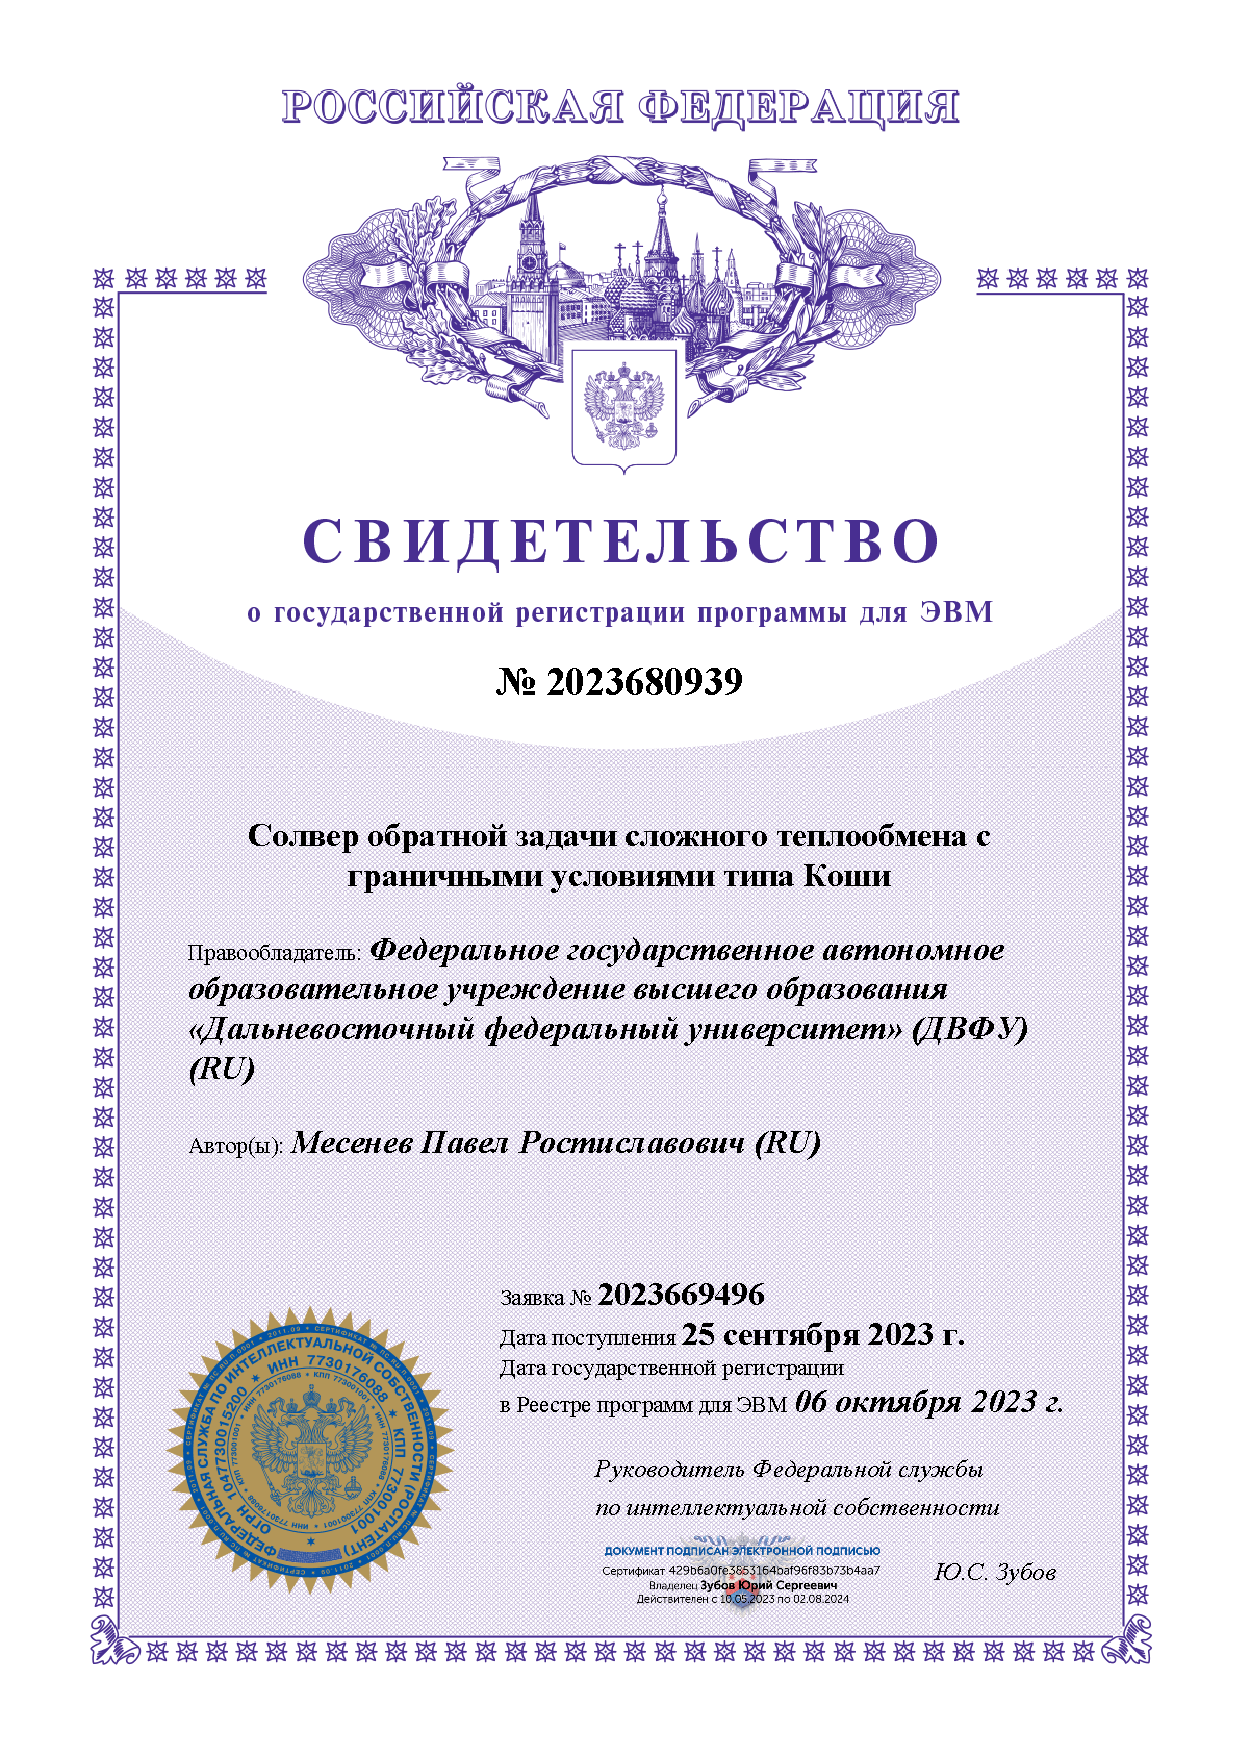
\includegraphics[width=1\linewidth]{reg1}}
    \end{minipage}
    \hfill
    \begin{minipage}[t]{0.3\linewidth}
        \center{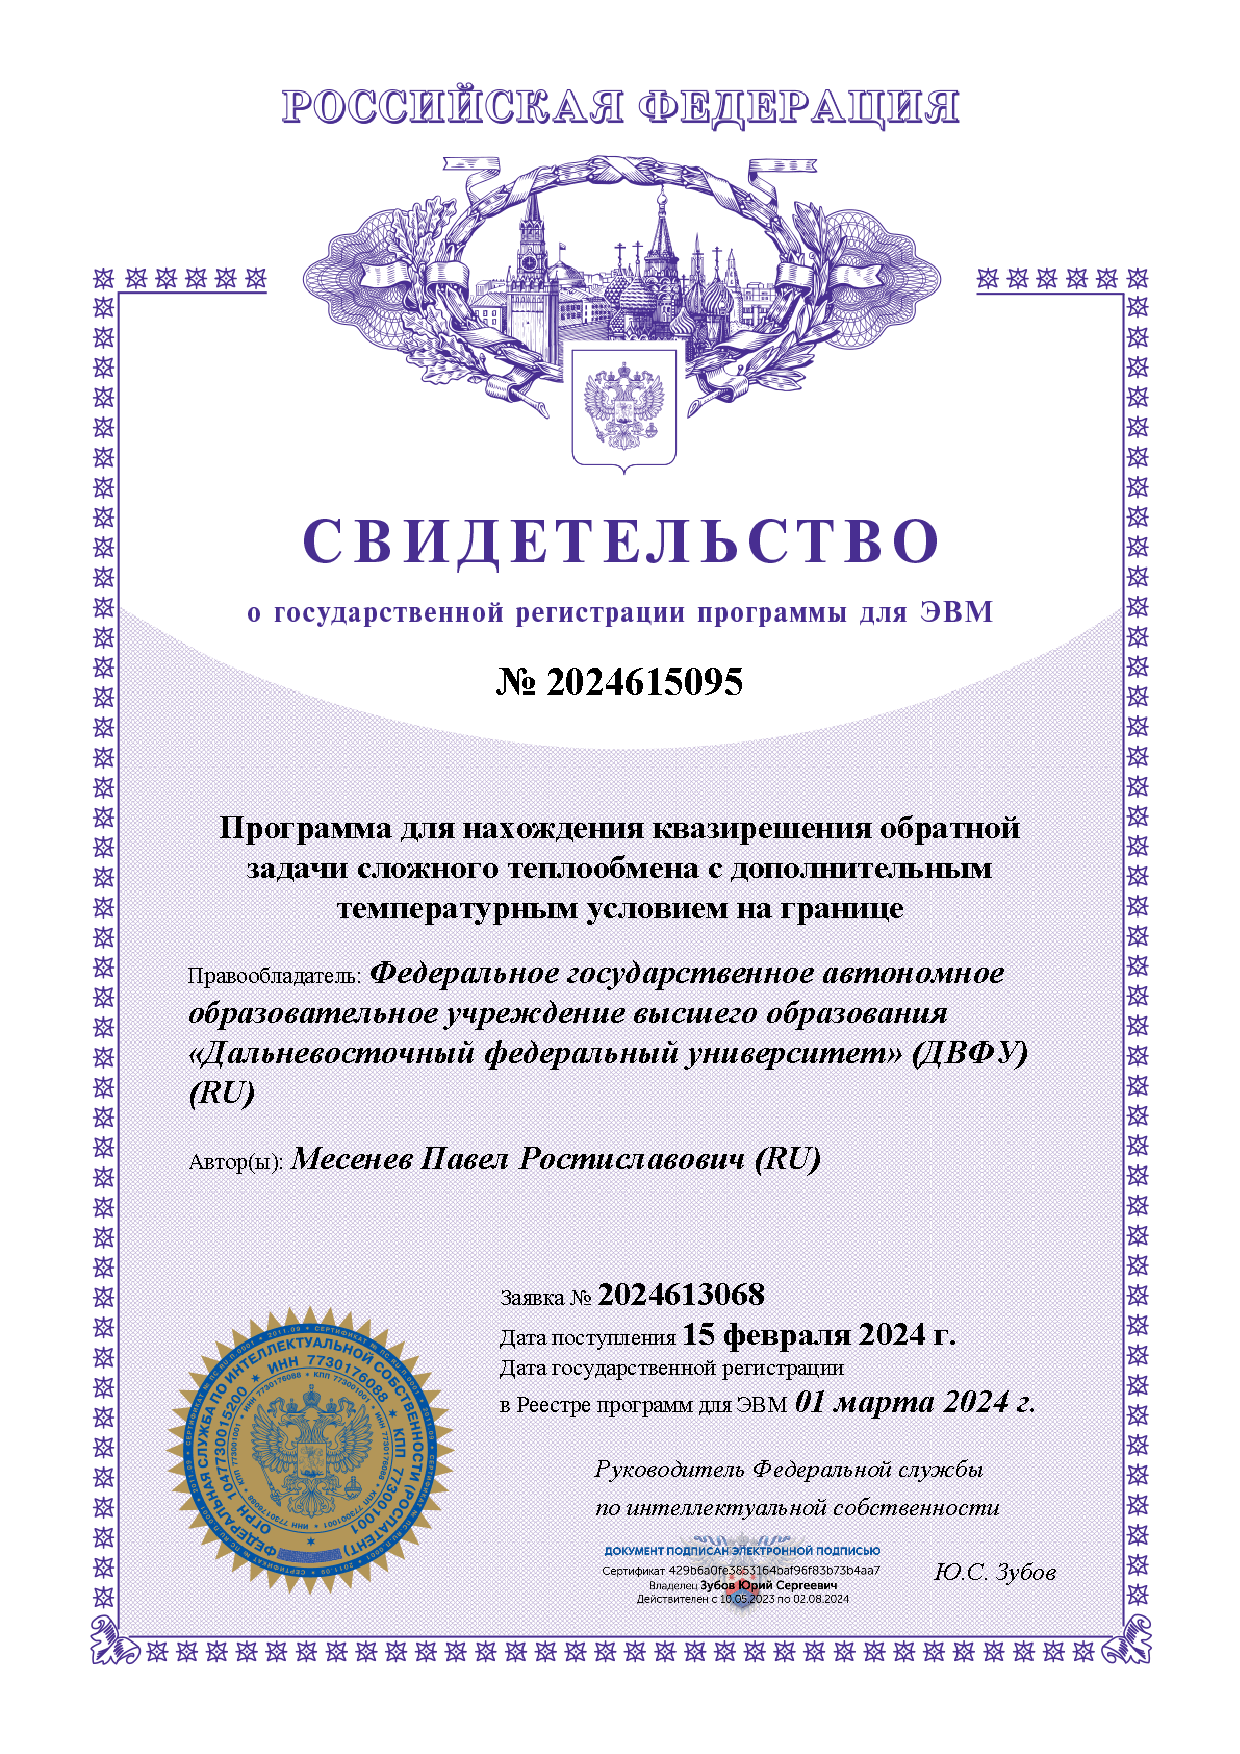
\includegraphics[width=1\linewidth]{reg2}}
    \end{minipage}
    \hfill
    \begin{minipage}[t]{0.3\linewidth}
        \center{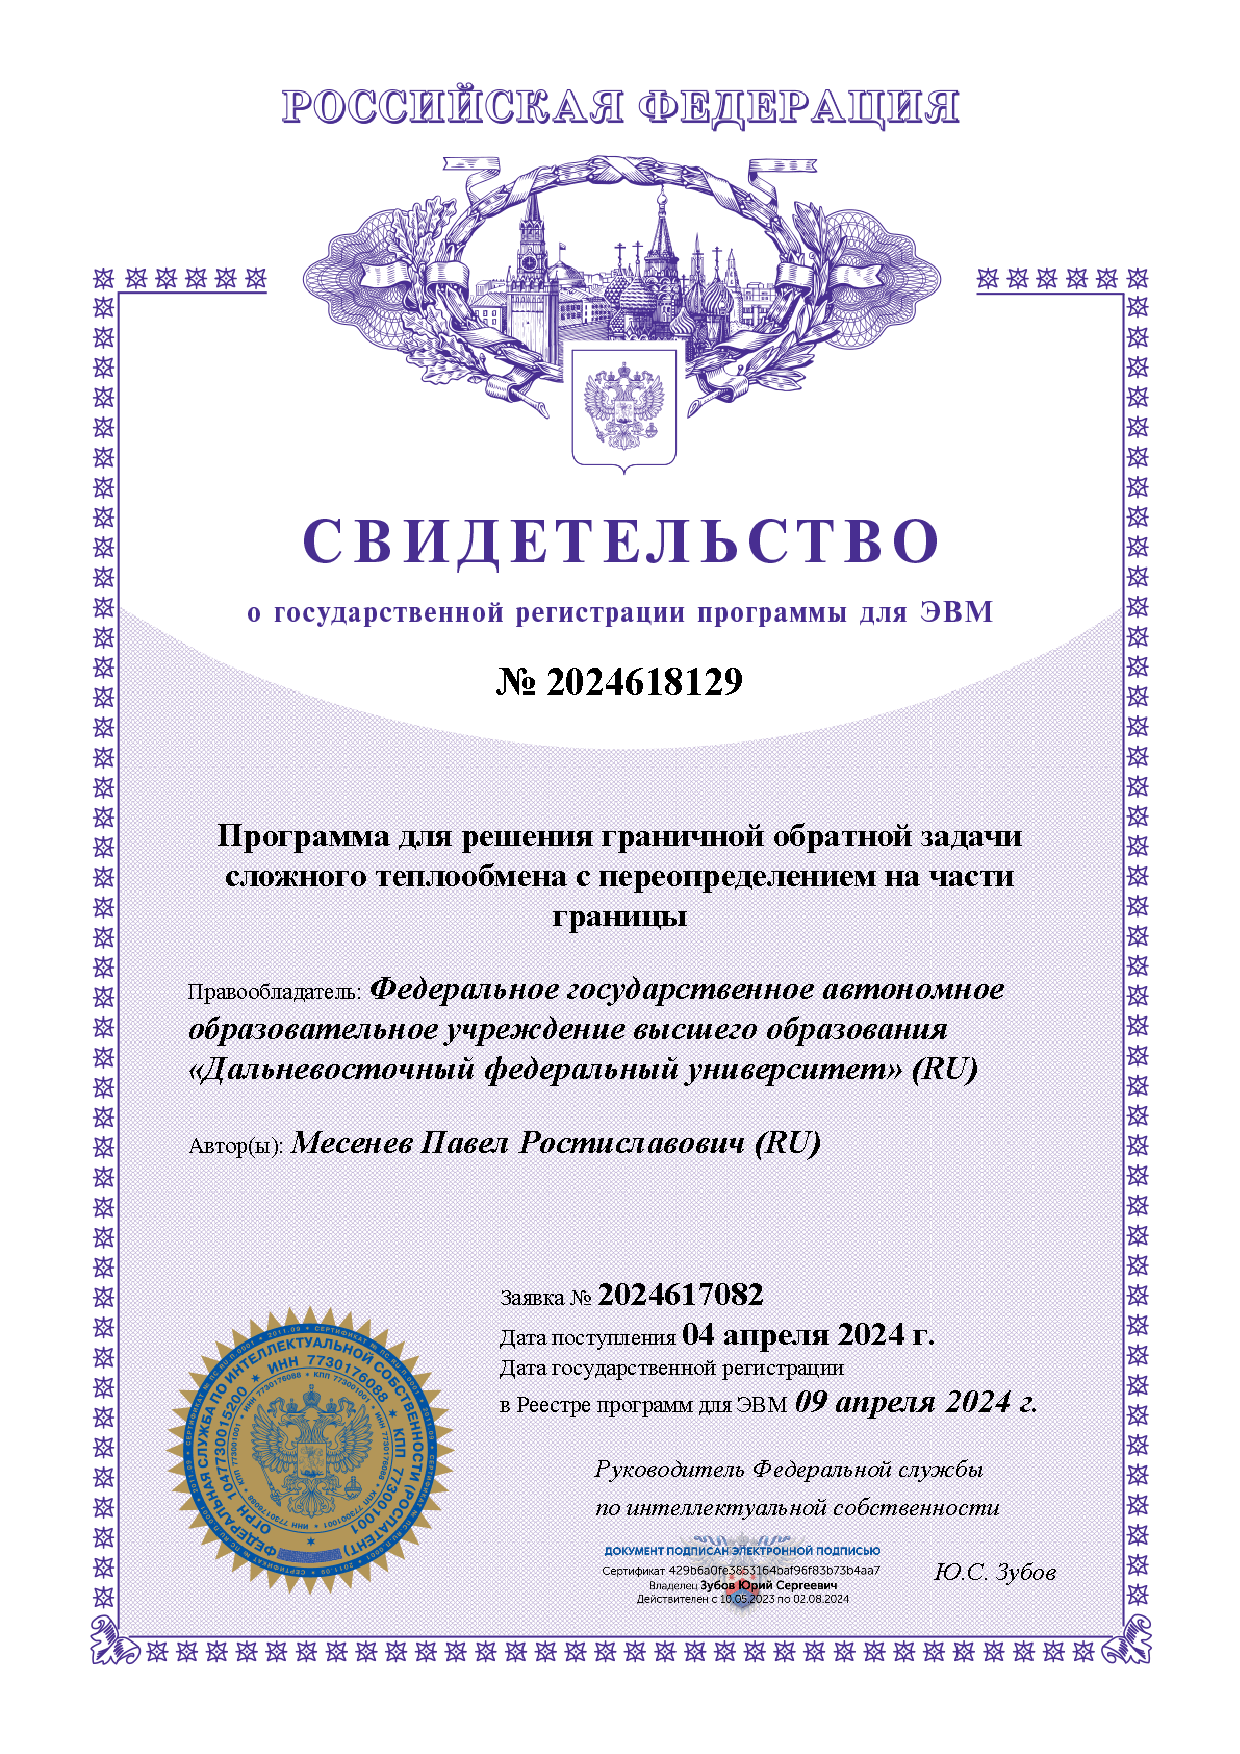
\includegraphics[width=1\linewidth]{reg3}}
    \end{minipage}
\end{frame}


\begin{frame} % публикации на одной странице
    \frametitle{Основные публикации}
    \small{
        \begin{enumerate}
            \item P. R. Mesenev. — «Optimization method for solving the inverse problem
            of complex heat transfer». —  \textit{Дальневост. матем. журн.} 23.1 (2023).
            \item A. Yu. Chebotarev, N. M. Park, P. R. Mesenev и A. E. Kovtanyuk. —
            «Penalty method to solve an optimal control problem for a quasilinear
            parabolic equation». —  \textit{Dal’nevostochnyi Matematicheskii Zhurnal} 22 (2022), с. 158—163.
            \item A. Yu. Chebotarev и P. R. Mesenev. — «An algorithm for solving
            the boundary value problem of radiation heat transfer without
            boundary conditions for radiation intensity». —  \textit{Dal’nevostochnyi
            Matematicheskii Zhurnal} (2020), с. 114—122.
            \item P. R. Mesenev и A. Yu. Chebotarev. — «A boundary inverse
            problem for complex heat transfer equations». — \textit{Dal’nevostochnyi
            Matematicheskii Zhurnal} 18.1 (2018), с. 75—84.
            \item П. Р. Месенев и А. Ю. Чеботарев. — «Задача сложного теплообмена с
            условиями типа Коши на части границы». — \textit{Ж. вычисл. матем. и матем. физ.}
            63.5 (2023), с. 856—863.
            \item P R Mesenev and A Yu Chebotarev. — “Analysis of an optimization
            method for solving the problem of complex heat transfer with Cauchy
            boundary conditions”. —  \textit{Comput. Math. Math. Phys. 62.1} (Jan. 2022).
        \end{enumerate}
    }
\end{frame}


\begin{frame}
    \frametitle{Участие в конференциях}
    \begin{itemize}
        \item Региональная научно-практическая конференция студентов, аспирантов
        и молодых учёных по естественным наукам (Владивосток, 2018, 2019);
        \item Workshop on Computing Technologies and Applied Mathematics
        (Вычислительные технологии и прикладная математика, Владивосток, 2022);
        \item International Conference DAYS on DIFFRACTION (Санкт-Петербург, 2021, 2023);
        \item International Workshop on Mathematical Modeling and Scientific Computing (Мюнхен, 2020, 2022).
    \end{itemize}
\end{frame}
